\documentclass[tikz, border=20pt]{standalone}
\usepackage{amsmath}

\begin{document}
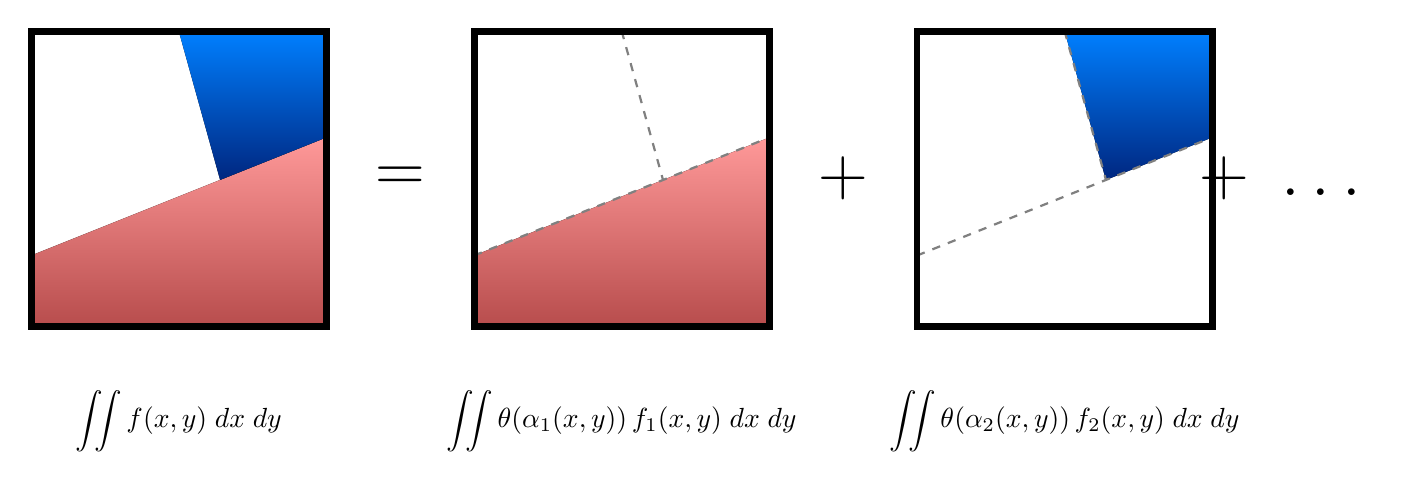
\begin{tikzpicture}[x=0.75cm, y=0.75cm]

    % ==========================================
    % MACRO: Define coordinates for the shapes
    % ==========================================
    \def\setcoords{
        \coordinate (RedL) at (0, 1.2);
        \coordinate (RedR) at (5, 3.2);
        \coordinate (SolidTop) at (2.5, 5);
        \coordinate (SolidBot) at (3.2, 2.48);
    }

    % ==========================================
    % PANEL 1: FULL PIXEL (The Total Integral)
    % ==========================================
    \begin{scope}[shift={(0,0)}]
        \setcoords
        \begin{scope}
            \clip (0,0) rectangle (5,5);
            % Bottom Region (Red)
            \fill[top color=red!40!white, bottom color=red!60!black!70]
                (0,0) -- (5,0) -- (RedR) -- (RedL) -- cycle;
            % Top Right Region (Blue)
            \fill[top color=blue!50!cyan, bottom color=blue!70!cyan!50!black]
                (SolidTop) -- (5,5) -- (5,3.2) -- (SolidBot) -- cycle;
        \end{scope}
        
        % Thick black border for the pixel
        \draw[line width=2.5pt, black] (0,0) rectangle (5,5);
        
        % Math Label
        \node[yshift=-1.2cm] at (2.5, 0) {$\displaystyle \iint f(x,y)\; dx\;dy$};
    \end{scope}

    % Math Operator
    \node at (6.25, 2.5) {\Huge $=$};

    % ==========================================
    % PANEL 2: FIRST TRIANGLE (Red Highlight)
    % ==========================================
    \begin{scope}[shift={(7.5,0)}]
        \setcoords
        \begin{scope}
            \clip (0,0) rectangle (5,5);
            % Fill only Red
            \fill[top color=red!40!white, bottom color=red!60!black!70]
                (0,0) -- (5,0) -- (RedR) -- (RedL) -- cycle;
        \end{scope}
        
        % Dashed boundaries to show the partition context
        \draw[gray, thick, dashed] (RedL) -- (RedR);
        \draw[gray, thick, dashed] (SolidTop) -- (SolidBot);

        % Thick black border
        \draw[line width=2.5pt, black] (0,0) rectangle (5,5);
        
        % Math Label
        \node[yshift=-1.2cm] at (2.5, 0) {$\displaystyle \iint \theta(\alpha_1(x,y))\,f_1(x,y)\; dx\;dy$};
    \end{scope}

    % Math Operator
    \node at (13.75, 2.5) {\Huge $+$};

    % ==========================================
    % PANEL 3: SECOND TRIANGLE (Blue Highlight)
    % ==========================================
    \begin{scope}[shift={(15,0)}]
        \setcoords
        \begin{scope}
            \clip (0,0) rectangle (5,5);
            % Fill only Blue
            \fill[top color=blue!50!cyan, bottom color=blue!70!cyan!50!black]
                (SolidTop) -- (5,5) -- (5,3.2) -- (SolidBot) -- cycle;
        \end{scope}
        
        % Dashed boundaries to show the partition context
        \draw[gray, thick, dashed] (RedL) -- (RedR);
        \draw[gray, thick, dashed] (SolidTop) -- (SolidBot);

        % Thick black border
        \draw[line width=2.5pt, black] (0,0) rectangle (5,5);
        
        % Math Label
        \node[yshift=-1.2cm] at (2.5, 0) {$\displaystyle \iint \theta(\alpha_2(x,y))\,f_2(x,y)\; dx\;dy$};
    \end{scope}

    % Math Operator (To represent the remaining empty white region)
    \node at (21.25, 2.5) {\Huge $+\ \dots$};

\end{tikzpicture}
\end{document}